\documentclass[aspectratio=169,10pt]{beamer}

% Compile with XeLaTeX or LuaLaTeX
\usepackage{fontspec}
\setmainfont{Fira Sans Light}

\usepackage{amsmath,amssymb,mathtools}
\usepackage{booktabs}
\usepackage{graphicx}
\usepackage{xcolor}

% Theme (research-like)
\usetheme{Madrid}
\usecolortheme{dolphin}
\setbeamertemplate{navigation symbols}{}

% Optional: slide numbers in the footer (clean + fits)
\setbeamertemplate{footline}{%
  \leavevmode%
  \hbox{%
    \begin{beamercolorbox}[wd=\paperwidth,ht=2.5ex,dp=1.2ex,leftskip=0.8em,rightskip=0.8em]{author in head/foot}%
      \hfill \insertframenumber{} / \inserttotalframenumber
    \end{beamercolorbox}%
  }%
}

% Title information
\title[Multi-objective Diet Optimization]{\LARGE Multi-objective Diet Optimization Problem}
\subtitle{\large Bioinspired Algorithms for Optimization 2026 - Group 11}
\author[De Los Santos \& Andonovski]{Ismael De Los Santos \and Gjorgi Andonovski}
\institute[]{\textbf{Professors:} Cristian Ramírez Atencia, Ángel Panizo LLedot \\[0.2cm] Universidad Politécnica de Madrid (UPM)}
\date{May 2026}

\begin{document}

% Title frame
\begin{frame}
    \titlepage
\end{frame}


%================================================
\begin{frame}
\frametitle{Problem Formulation}

\textbf{Goal.} Design 7-day meal plans minimizing two conflicting objectives: caloric deviation and macronutrient imbalance.

\vspace{0.3cm}

\textbf{Problem parameters.}
\begin{itemize}
  \item Catalogue of 2,616 real food items with complete nutritional data.
  \item Five user profiles spanning ages 17 to 72, with daily caloric targets from 1,401 to 3,103 kcal.
  \item Weekly schedule: 7 days $\times$ 11 meal slots per day = 77 decision variables.
  \item Each slot restricted to an admissible set $D_j$ (e.g., snacks limited to fruits and sugars; breakfast/lunch/dinner split into drink and solid slots).
\end{itemize}

\vspace{0.3cm}

\textbf{Multi-objective model.}
\begin{align}
\min\ f_1(\mathbf{x}) &= \sum_{d=1}^{7} |K(\mathbf{x},d) - T| \quad \text{(caloric balance)} \\
\min\ f_2(\mathbf{x}) &= \sum_{d=1}^{7} (|p_C - 50| + |p_F - 27.5| + |p_P - 22.5|) \quad \text{(macronutrient balance)}
\end{align}
subject to $x_j \in D_j$ for all $j = 1, \ldots, 77$.

\end{frame}

%================================================
\begin{frame}
\frametitle{Solution Representation}

\textbf{Two encodings tested.}

\vspace{0.2cm}

\textbf{Direct-Index.} A length-77 integer vector where gene $j$ directly stores the food ID assigned to slot $j$:
\[
\mathbf{x} \in \{1, \ldots, 2616\}^{77}.
\]
The generator samples each gene uniformly from its domain $D_j$. Mutation replaces a selected gene with a fresh uniform draw from $D_j$. Crossover uses multi-point recombination, and since both parents are feasible and values are copied position-wise, offspring remain feasible.

\vspace{0.3cm}

\textbf{Random-Key.} A length-77 real vector where each component is decoded to a food ID:
\[
\mathbf{k} \in [0,1]^{77}.
\]
For each position $j$, the interval $[0,1]$ is partitioned into $|D_j|$ equal-width bins, and $k_j$ selects the corresponding domain element. This guarantees that any key vector in $[0,1]^{77}$ decodes to a feasible direct-index plan. Mutation perturbs selected keys with Gaussian noise ($\sigma = 0.1$) and clamps to $[0,1]$. Crossover applies multi-point recombination in key space.

\vspace{0.2cm}

\textbf{Feasibility-preserving design:} Both encodings enforce slot-wise feasibility by construction; constraints are never violated.

\end{frame}

%================================================
\begin{frame}
\frametitle{Fitness Evaluation}

\textbf{For each weekly plan $\mathbf{x}$:}

\vspace{0.2cm}

For every day $d \in \{1, \ldots, 7\}$:
\begin{enumerate}
  \item Aggregate energy and macronutrient content from the 11 food items assigned to that day.
  \item Compute total daily caloric intake $K(\mathbf{x}, d)$ (in kcal).
  \item Calculate macronutrient energy percentages using Atwater conversion factors: $K_C = 4C$, $K_F = 9F$, $K_P = 4P$.
  \item Compute daily macronutrient energy shares: $p_M(\mathbf{x}, d) = 100 \cdot K_M(\mathbf{x}, d) / K(\mathbf{x}, d)$ for $M \in \{C, F, P\}$.
  \item Accumulate deviations.
\end{enumerate}

\vspace{0.2cm}

Final objectives:
\begin{itemize}
  \item $f_1 = \sum_{d=1}^{7} |K(\mathbf{x}, d) - T|$ (total weekly kcal deviation).
  \item $f_2 = \sum_{d=1}^{7} (|p_C - 50| + |p_F - 27.5| + |p_P - 22.5|)$ (daily percentage deviations aggregated).
\end{itemize}

\vspace{0.2cm}

Pareto dominance comparison: a solution dominates another if it is better or equal in both objectives, and strictly better in at least one.

\end{frame}

%================================================
\begin{frame}
\frametitle{Algorithms: NSGA-II and PAES}

\textbf{NSGA-II (Non-dominated Sorting GA-II).}
\begin{itemize}
  \item Population-based evolutionary algorithm with population size 80 and 80 generations.
  \item Non-dominated sorting ranks solutions into fronts; crowding distance maintains diversity within each front.
  \item Tested with both direct-index and random-key encodings.
  \item Mutation: domain-aware discrete mutation on direct-index; Gaussian perturbation on random-key.
  \item Crossover: multi-point crossover on both encodings.
\end{itemize}

\vspace{0.3cm}

\textbf{PAES (Pareto Archived Evolution Strategy).}
\begin{itemize}
  \item Single-solution (1+1) evolution strategy with adaptive grid archive.
  \item Population size fixed at 1; 800 generations to compensate for single-solution trajectory.
  \item Archive-driven acceptance: new solutions accepted if they improve the archive coverage.
  \item Direct-index encoding only.
  \item Archive size 40; mutation rate 0.1.
\end{itemize}

\end{frame}

%================================================
\begin{frame}
\frametitle{Algorithms: MOPSO and P-ACO}

\textbf{MOPSO (Multi-Objective Particle Swarm Optimizer).}
\begin{itemize}
  \item Particle swarm operating in random-key continuous space ($[0,1]^{77}$).
  \item Population 30, 80 generations; particles guided by leaders selected from an external non-dominated archive.
  \item Leader selection via Mostaghim-Teich sigma rule: solutions in sparse regions preferred.
  \item Archive bounded and pruned by crowding distance; particles updated with standard PSO velocity equations.
\end{itemize}

\vspace{0.3cm}

\textbf{P-ACO (Pareto Ant-Colony Optimization).}
\begin{itemize}
  \item Ants construct solutions by sequentially filling slots; each slot sampled from domain $D_j$ via pheromone-weighted categorical distribution.
  \item Population 60 ants, 40 generations.
  \item Direct-index space; pheromone reinforced from archive members (not from single best solution).
  \item Pheromone deposits weighted by crowding distance to favour diverse archive solutions.
  \item Evaporation and bounded pheromone levels control exploration.
\end{itemize}

\end{frame}

%================================================
\begin{frame}
\frametitle{Experimental Design}

\textbf{Hyperparameter tuning phase.}
\begin{itemize}
  \item Two representative subjects (subject 1: highest target; subject 4: mid-range target).
  \item Per-algorithm grid: 12--16 cells, 5 replicates each.
  \item Total: 56 cells $\times$ 4 algorithms $\times$ 5 replicates = 560 tuning runs.
  \item Hyperparameters selected by highest mean hypervolume.
\end{itemize}

\vspace{0.3cm}

\textbf{Full benchmark phase.}
\begin{itemize}
  \item Five configurations: NSGA-II (direct-index and random-key), PAES, MOPSO, P-ACO.
  \item All five user profiles (ages 17, 30, 40, 55, 72).
  \item 30 stochastic replicates per configuration (paired deterministic seeds).
  \item \textbf{Total: $5 \times 5 \times 30 = 750$ runs}.
\end{itemize}

\vspace{0.3cm}

\textbf{Metrics.} Hypervolume, IGD, Schott's spacing, Deb's $\Delta$-spread, best $f_1$, best $f_2$, runtime, front/archive size.

\textbf{Statistical tests.} Wilcoxon signed-ranks (pairwise) and Friedman aligned ranks (omnibus), with Shaffer post-hoc correction.

\end{frame}

%================================================
\begin{frame}
\frametitle{Hyperparameter Settings}

\begin{table}
\centering\small
\begin{tabular}{llrr}
\toprule
\textbf{Algorithm} & \textbf{Settings Selected} & \textbf{HV (tuning)} & \textbf{Rt (s)} \\
\midrule
NSGA-II & pop=80, gen=80, mut=0.2 & 969,654 & 1.39 \\
PAES & gen=800, archive=40, mut=0.1 & 474,575 & 1.93 \\
MOPSO & pop=30, gen=80, archive=80, $w=0.4$, $c_1=c_2=2.0$ & 489,401 & 0.30 \\
P-ACO & pop=60, gen=40, archive=40, $\rho=0.1$ & 459,679 & 22.69 \\
\bottomrule
\end{tabular}
\caption{Tuning winners from the hyperparameter sweep. PAES uses a (1+1)-ES so population is 1 by construction.}
\end{table}

\end{frame}

%================================================
\begin{frame}
\frametitle{Aggregated Results}

\begin{table}
\centering\small
\begin{tabular}{lrrrrrr}
\toprule
\textbf{Config} & \textbf{HV} & \textbf{IGD} & \textbf{$f_1$ best} & \textbf{$f_2$ best} & \textbf{Rt (s)} & \textbf{Front} \\
\midrule
NSGA-II DI & 1,014,630 & 171.75 & 1,343.37 & 167.77 & 1.38 & 80.00 \\
NSGA-II RK & 1,059,760 & 120.20 & 1,105.10 & 167.11 & 1.46 & 80.00 \\
PAES DI & 401,023 & 438.80 & 1,987.88 & 123.92 & 1.94 & 38.89 \\
MOPSO RK & 403,726 & 640.46 & 2,362.58 & 175.30 & 0.37 & 17.95 \\
P-ACO DI & 435,310 & 783.09 & 2,700.35 & 179.80 & 33.50 & 9.13 \\
\bottomrule
\end{tabular}
\caption{Mean metrics per configuration over $n=150$ runs (30 replicates $\times$ 5 subjects).}
\end{table}

\vspace{0.3cm}

\textbf{Key observations.}
\begin{itemize}
  \item NSGA-II (both encodings) dominates on Pareto coverage (HV and IGD).
  \item PAES achieves the lowest macronutrient deviation ($f_2 = 123.92$) but narrower Pareto front.
  \item MOPSO is the fastest (0.37 s) but mid-range quality.
  \item P-ACO achieves competitive hypervolume (435,310) but with substantial runtime overhead (33.50 s).
\end{itemize}

\end{frame}

%================================================
\begin{frame}
\frametitle{Statistical Significance Tests}

\textbf{Friedman Aligned Ranks (omnibus test).}
\begin{itemize}
  \item Hypervolume: $T = 585.92$, $p < 10^{-70}$.
  \item IGD: $T = 643.99$, $p < 10^{-70}$.
  \item Runtime: $T = 870.80$, $p < 10^{-70}$.
\end{itemize}

All metrics show highly significant differences across algorithms.

\vspace{0.3cm}

\textbf{Pairwise Wilcoxon Signed-Ranks with Shaffer Correction.}
\begin{itemize}
  \item Both NSGA-II variants significantly better on HV than PAES, MOPSO, P-ACO (all adjusted $p$-values $< 0.05$).
  \item NSGA-II encodings: no significant difference on HV ($p = 0.359$).
  \item Non-NSGA-II methods: not significantly different from one another on HV after Shaffer correction.
\end{itemize}

\vspace{0.3cm}

\textbf{Conclusion.} NSGA-II's superiority on Pareto front coverage is statistically proven. Encoding choice is not critical.

\end{frame}

%================================================
\begin{frame}
\frametitle{Hypervolume Distribution Across Configurations}
\centering

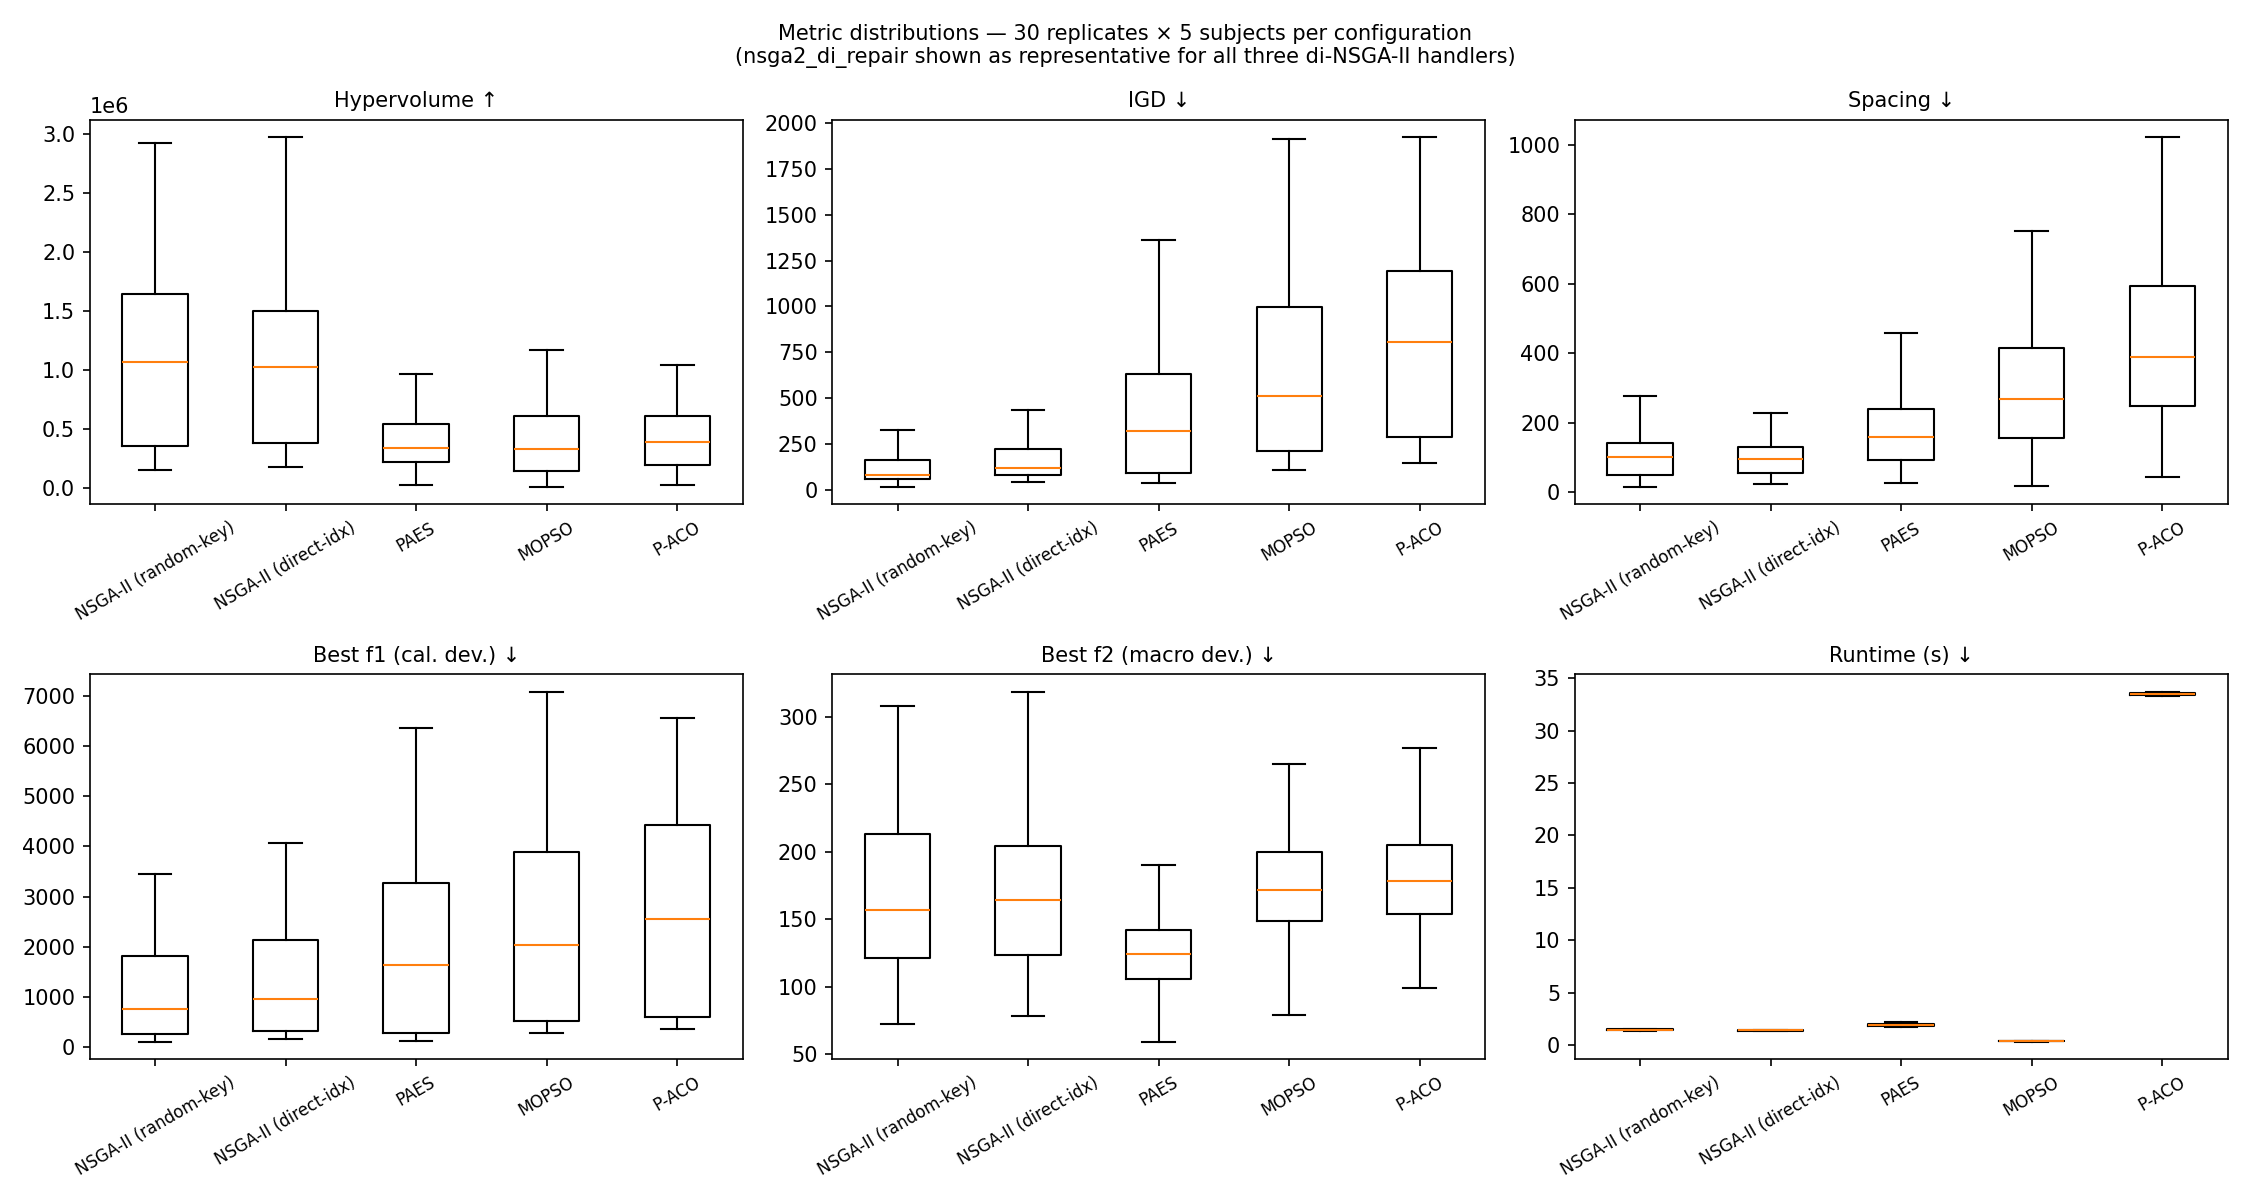
\includegraphics[width=0.92\linewidth,height=0.78\textheight,keepaspectratio]{experiments/boxplots.png}

\vspace{0.2cm}
\scriptsize Boxplots across 30 replicates $\times$ 5 subjects ($n=150$ per configuration).
\end{frame}

%================================================
\begin{frame}
\frametitle{Convergence and Diversity Overview}
\centering
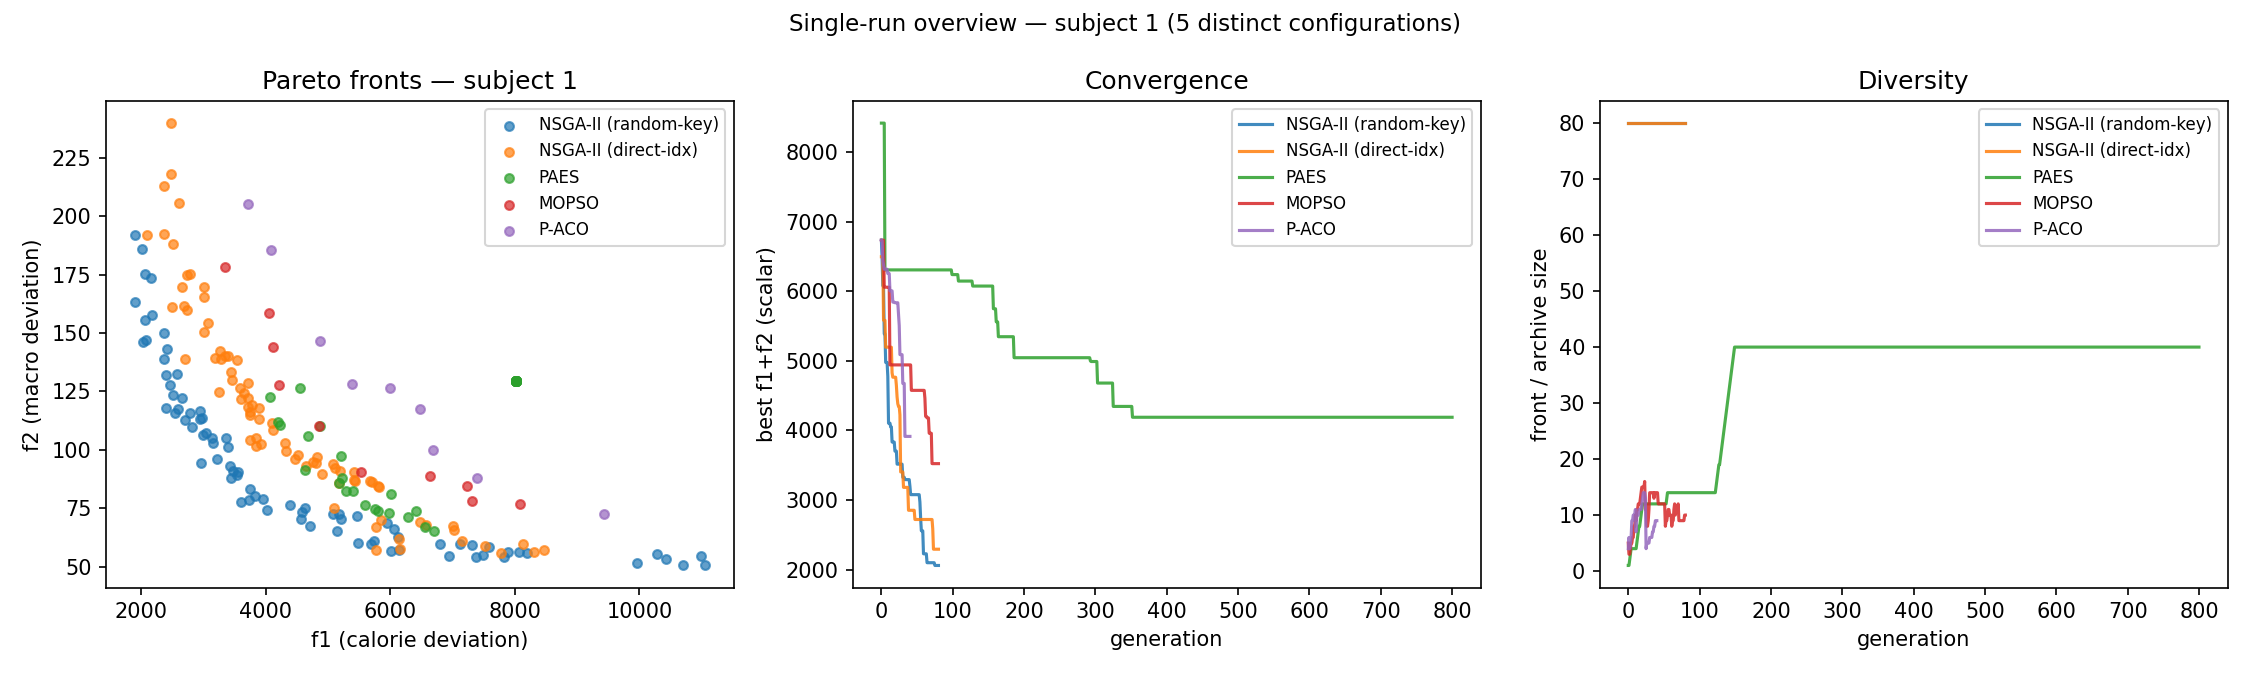
\includegraphics[width=0.92\linewidth,height=0.82\textheight,keepaspectratio]{experiments/demo_overview.png}
\end{frame}

%================================================
\begin{frame}
\frametitle{Objective-Space Analysis}

\begin{table}
\centering\small
\begin{tabular}{lrrr}
\toprule
\textbf{Config} & \textbf{Best $f_1$} & \textbf{Best $f_2$} & \textbf{Ratio $f_2/f_1$} \\
\midrule
NSGA-II RK & 1,105.10 & 167.11 & 0.151 \\
NSGA-II DI & 1,343.37 & 167.77 & 0.125 \\
PAES DI & 1,987.88 & 123.92 & 0.062 \\
MOPSO RK & 2,362.58 & 175.30 & 0.074 \\
P-ACO DI & 2,700.35 & 179.80 & 0.067 \\
\bottomrule
\end{tabular}
\caption{Single-objective performance: best achieved values for each objective.}
\end{table}

\vspace{0.2cm}

\textbf{Algorithmic specialization.}
\begin{itemize}
  \item NSGA-II excels at caloric balance ($f_1$) via crowding-distance diversity maintenance; balanced front achieves both objectives simultaneously.
  \item PAES specializes in macronutrient accuracy ($f_2 = 123.92$) at the cost of weaker caloric balance; archive-driven single-trajectory focuses deep exploration in one region.
  \item Swarm methods show intermediate patterns: MOPSO trades quality for speed; P-ACO balances both but slower.
\end{itemize}

\end{frame}

%================================================
\begin{frame}
\frametitle{Algorithm Design Insights}

\textbf{Feasibility-preserving encoding.}
\begin{itemize}
  \item Generator and all variators only sample from admissible domains $D_j$.
  \item Zero infeasible solutions ever produced.
  \item No constraint-handling overhead (no repair, penalty, or death penalty methods needed).
  \item This design choice streamlines search by eliminating post-hoc constraint management.
\end{itemize}

\vspace{0.3cm}

\textbf{Performance drivers.}
\begin{itemize}
  \item \textbf{NSGA-II:} Non-dominated sorting and crowding distance maintain a diverse approximation to the full Pareto trade-off surface without requiring problem-specific distance metrics.
  \item \textbf{PAES:} Archive-driven single-solution trajectory allows deep exploitation but at the cost of broader coverage.
  \item \textbf{MOPSO:} Continuous velocity updates through random-key decoding enable fast convergence but reduced precision on discrete food assignments.
  \item \textbf{P-ACO:} Pheromone learning from archive members captures combinatorial structure but requires careful vectorization for efficiency.
\end{itemize}

\vspace{0.2cm}

\textbf{Critical observation.} Encoding choice (direct-index vs random-key) does not significantly impact solution quality; algorithm paradigm (evolutionary vs swarm) is the dominant factor.

\end{frame}

%================================================
\begin{frame}
\frametitle{Conclusions}

\begin{itemize}
  \item \textbf{Best overall:} NSGA-II with direct-index encoding delivers strong Pareto coverage (HV 1,014,630) with slightly better runtime (1.38 s) than random-key.

  \vspace{0.25cm}

  \item \textbf{Alternative configurations:}
  \begin{itemize}
    \item PAES if obtaining a single macronutrient-optimal plan is the primary goal ($f_2 = 123.92$).
    \item MOPSO if runtime is the critical constraint (0.37 s per run).
  \end{itemize}

  \vspace{0.25cm}

  \item \textbf{Key design principle:} Feasibility-preserving encoding eliminates constraint-handling overhead, simplifying both the fitness evaluation and the algorithmic implementation.

  \vspace{0.25cm}

  \item \textbf{Multi-objective framework:} Pareto dominance naturally balances conflicting objectives (caloric vs macronutrient) without scalarization or user-defined weights.

  \vspace{0.25cm}

  \item \textbf{Statistical validation:} Friedman and Wilcoxon tests confirm that NSGA-II's superiority is not by chance ($p < 10^{-70}$).
\end{itemize}

\end{frame}

\end{document}